\documentclass[UTF8,a4paper,12pt]{ctexart}

% =========================
% 基础宏包
% =========================
\usepackage{geometry}
\usepackage{setspace}
\usepackage{graphicx}
\usepackage{float}
\usepackage{booktabs}
\usepackage{array}
\usepackage{longtable}
\usepackage{tabularx}
\usepackage{multirow}
\usepackage{enumitem}
\usepackage{xcolor}
\usepackage{listings}
\usepackage{hyperref}
\usepackage{caption}
\usepackage{subcaption}
\usepackage{amsmath}
\usepackage{amssymb}
\usepackage{tikz}
\usepackage{makecell}
\usepackage{fancyhdr}
\usepackage{graphicx} % 必须引入

% =========================
% 页面设置
% =========================
\geometry{
    left=2.6cm,
    right=2.6cm,
    top=2.5cm,
    bottom=2.5cm
}

\setstretch{1.35}
\setcounter{tocdepth}{2}
\setcounter{secnumdepth}{3}
\emergencystretch=2em
\setlength{\headheight}{15pt}

% =========================
% 页眉页脚
% =========================
\pagestyle{fancy}
\fancyhf{}
\fancyhead[L]{编译原理课程大作业 2 设计报告}
\fancyhead[R]{类 Rust 语义分析与中间代码生成}
\fancyfoot[C]{\thepage}

% =========================
% 超链接设置
% =========================
\hypersetup{
    colorlinks=true,
    linkcolor=black,
    urlcolor=blue,
    citecolor=black,
    plainpages=false
}

% =========================
% TikZ 设置
% =========================
\usetikzlibrary{arrows.meta,positioning,shapes.geometric,fit,calc}
\tikzset{
    box/.style={
        draw,
        rounded corners,
        align=center,
        minimum height=9mm,
        minimum width=24mm,
        fill=blue!6
    },
    bigbox/.style={
        draw,
        rounded corners,
        align=center,
        minimum height=11mm,
        minimum width=32mm,
        fill=green!8
    },
    flow/.style={-Latex, thick},
    decision/.style={
        draw,
        diamond,
        aspect=2,
        align=center,
        inner sep=1pt,
        fill=orange!10
    }
}

% =========================
% 代码块设置
% =========================
\lstdefinelanguage{Rust}{
    keywords={fn,let,mut,if,else,while,for,in,loop,break,continue,return,match,enum,struct,impl,trait,mod,use,pub,crate,super,Self,self,as,ref},
    sensitive=true,
    morecomment=[l]{//},
    morecomment=[s]{/*}{*/},
    morestring=[b]"
}

\lstdefinestyle{codeStyle}{
    basicstyle=\ttfamily\fontsize{8.5pt}{9.7pt}\selectfont,
    numbers=left,
    numberstyle=\tiny,
    stepnumber=1,
    numbersep=8pt,
    frame=single,
    breaklines=true,
    tabsize=4,
    showstringspaces=false,
    keywordstyle=\color{blue},
    commentstyle=\color{gray},
    stringstyle=\color{teal},
    columns=fullflexible
}

\lstdefinestyle{textStyle}{
    basicstyle=\ttfamily\fontsize{8.5pt}{9.7pt}\selectfont,
    frame=single,
    breaklines=true,
    showstringspaces=false,
    columns=fullflexible
}

\lstset{style=codeStyle}

% =========================
% 表格列格式
% =========================
\newcolumntype{Y}{>{\raggedright\arraybackslash}X}
\newcolumntype{P}[1]{>{\raggedright\arraybackslash}p{#1}}

% =========================
% 自定义命令
% =========================
\newcommand{\pkg}[1]{\texttt{#1}}
\newcommand{\ruleid}[1]{\textbf{#1}}
\newcommand{\op}[1]{\texttt{#1}}

% =========================
% 文档信息
% =========================
\begin{document}

% =========================
% 封面
% =========================
\pagenumbering{Roman}
\begin{titlepage}
    \thispagestyle{empty}
    \centering

    \vspace*{0.8cm}
    
\includegraphics[width=0.18\textwidth]{figures/tongji.png}\par

    \vspace{0.9cm}
    {\heiti\zihao{2} 同济大学编译原理课程大作业 2\par}

    \vspace{1.1cm}
    {\heiti\zihao{1} 设计报告\par}

    \vspace{0.8cm}
    {\zihao{-2} 类 Rust 语言语义分析与四元式\par}
    {\zihao{-2} 中间代码生成器设计与实现\par}

    \vfill
    \renewcommand{\arraystretch}{1.7}
    \begin{tabular}{rl}
        学院： & 计算机科学与技术学院 \\
        专业： & 计算机科学与技术 \\
        小组成员： & 白佳煜、胡桥健、庄子硕 \\
        学号： & 2352733、2351295、2350998 \\
        指导教师： & 卫志华、高珍 \\
    \end{tabular}

    \vfill
    {\zihao{4} \today\par}
\end{titlepage}

\setcounter{page}{2}
\pdfbookmark[1]{目录}{toc}
\tableofcontents
\clearpage
\pagenumbering{arabic}
\setcounter{page}{1}

% =========================
% 正文
% =========================

\section{实验背景与任务要求}

\subsection{实验背景}

编译器前端在完成词法分析和语法分析之后，还需要继续回答两个更接近“可执行语义”的问题：第一，源程序在静态语义层面是否成立；第二，若程序成立，应当如何将它翻译为后续优化、解释或目标代码生成更容易处理的中间形式。课程大作业 1 已经围绕类 Rust 语言完成了词法分析器与语法分析器的实现，形成了从源程序到抽象语法树（AST）的基础流水线。大作业 2 则在此基础上继续向后推进，要求实现语义分析与中间代码生成器，使系统从“会读代码”进一步演进为“能理解代码并给出结构化翻译结果”。

从编译原理角度看，语义分析阶段负责处理上下文相关的信息，包括符号是否声明、作用域嵌套、类型是否匹配、不可变变量是否被二次赋值、循环控制语句是否出现在合法位置、函数调用实参与形参是否一致等。与词法分析和语法分析相比，这一阶段不再仅仅依赖局部模式匹配，而是需要显式维护环境、上下文、属性与约束关系。中间代码生成则要求编译器把较复杂的语法结构转换成形式更统一、控制流更清晰的表示。本项目最终选择四元式作为中间代码形式，以兼顾课程展示的直观性、实现复杂度与可测试性。

Rust 语言本身具有鲜明的静态语义特征，例如显式的可变性、引用与借用约束、表达式块、数组与元组等。课程给出的类 Rust 语法在保留这些关键思想的同时，又将语言规模控制在教学实验可完成的范围内。因此，本项目既需要满足课程作业中强制规定的最低规则集合，又应尽可能在工程上扩展更多语法和语义能力，体现对现代编程语言静态语义设计的理解。

\subsection{作业二的核心目标}

根据 \pkg{Resources/Task2/【Rust版】大作业2：中间代码生成器.pptx} 的要求，本次大作业的直接目标可以概括为以下四点：

\begin{enumerate}[label=\arabic*.]
    \item 在既有 AST 基础上实现类 Rust 语言的静态语义分析，能够识别变量、函数、表达式、控制流和复合数据结构中的语义错误；
    \item 以四元式形式生成中间代码，覆盖函数、赋值、算术运算、比较运算、条件分支、循环、数组、元组等构造；
    \item 对静态语义错误进行诊断并保留尽可能完整的上下文信息，使结果既可用于自动化测试，也适合课程答辩中的人工检查；
    \item 在基础要求之上，讨论更通行的高级语言语义问题，如严格条件类型、表达式块、引用与借用、错误恢复、边界检查以及工程化测试策略。
\end{enumerate}

作业说明强调了“语义分析结果”和“中间代码生成”两个并列目标，这意味着系统不能只在出错时停在诊断层面，也不能只在成功时生成若干理想化四元式。更合理的工程目标应当是：在语义合法时生成正确、稳定、可解释的中间代码；在语义不合法时尽可能报告有辨识度的错误，并在不引发连锁污染的前提下保持中间结果的可观察性。

\subsection{最低强制规则范围}

PPT 第 25 页明确给出了本次作业的最低完成规则范围。它们构成课程验收的硬性基础，也是本文报告重点论述的部分。表 \ref{tab:mandatory-rules-overview} 给出了这些规则的编号与含义概览。

\begin{table}[H]
    \centering
    \caption{作业二强制完成规则概览}
    \label{tab:mandatory-rules-overview}
    \begin{tabularx}{\textwidth}{P{2cm}Y}
        \toprule
        规则编号 & 规则内容 \\
        \midrule
        0.1, 0.2, 0.3 & \pkg{mut} 变量属性、\pkg{i32} 基础类型、左值/可取引用/可取元素 \\
        1.1, 1.2, 1.3, 1.4, 1.5 & 基础程序结构、空语句、\pkg{return;}、函数输入、函数输出 \\
        2.0, 2.1, 2.2 & 变量声明、变量声明语句、赋值语句 \\
        3.1, 3.2, 3.3, 3.4, 3.5 & 基本表达式、比较运算、加减运算、乘除运算、函数调用 \\
        4.1 & \pkg{if} 选择结构 \\
        5.0, 5.1 & 循环语句框架与 \pkg{while} 循环 \\
        \bottomrule
    \end{tabularx}
\end{table}

从规则依赖关系可以看到，课程采用了一种自底向上的增量式设计：先给出变量属性、类型与左值概念，再建立函数和语句框架，随后补充表达式、条件与循环。在这种组织方式下，语义分析器的正确性不仅体现在单条规则是否实现，还体现在规则之间能否协同工作。例如，函数调用规则依赖于函数签名表、参数类型检查和返回值类型传播；\pkg{while} 规则依赖于条件表达式求值与循环上下文管理。

\subsection{评分标准与报告要求}

PPT 第 24 页给出了大作业 2 的评分标准，第 25 页给出了交付物要求。评分并不只看功能是否“跑通”，而是同时考察问题分析能力、系统设计能力、编程能力、报告质量和文献检索能力。因此，报告不能仅列出“实现了哪些规则”，而应完整说明如下内容：

\begin{itemize}
    \item 为什么需要这些语义规则，它们与编译原理中的静态语义、属性文法、作用域与类型系统有何关系；
    \item 系统整体如何分层组织，各模块之间怎样传递数据，为什么选择四元式而不是其他中间表示；
    \item 每一类语义检查如何落在具体代码中，如何处理错误恢复，如何保证后续四元式仍可观测；
    \item 典型测试程序与结果如何设计，哪些例子来自课程 PPT，哪些例子用于扩展规则或边界场景；
    \item 当前实现有哪些不足，哪些是刻意的课程级简化，哪些是后续可以继续工程化增强的方向。
\end{itemize}

课程还要求报告中给出程序实例与结果截屏。考虑到当前仓库已经提供 Web 可视化界面，且本项目更关注结构性分析结果，本文在截图之外额外使用多幅结构图、控制流图和四元式模板图，目的是把“程序运行结果”与“设计本身”同时展示清楚，避免报告沦为简单的功能说明书。

\section{当前实现概况与仓库结构}

\subsection{仓库总体结构}

当前仓库不是单一的 Cargo workspace，而是由四个 Rust crate 和一个前端页面共同组成。仓库根目录中的 \pkg{README.md} 对此做了较新的说明，且其内容与源码结构一致。表 \ref{tab:repo-structure} 概括了各部分的职责。

\begin{table}[H]
    \centering
    \caption{仓库主要组成部分}
    \label{tab:repo-structure}
    \begin{tabularx}{\textwidth}{P{3cm}Y Y}
        \toprule
        目录或文件 & 职责定位 & 主要产出 \\
        \midrule
        \pkg{Easy\_Lexer} & 词法分析，识别关键字、标识符、数字、算符与界符，并报告词法错误 & token 序列、词法错误 \\
        \pkg{Easy\_Parser} & 递归下降语法分析，构建 JSON 可序列化的 AST & \pkg{Program} AST、语法错误 \\
        \pkg{Easy\_Analyzer} & 语义分析与四元式生成，是作业二的核心实现 & 语义错误、四元式序列 \\
        \pkg{Easy\_Server} & 本地 Web 服务，聚合 lexer、parser 与 analyzer 结果 & Web API 响应、可视化数据 \\
        \pkg{index.html} & 前端页面，展示 token 表、AST 树、四元式与错误信息 & 浏览器交互界面 \\
        \pkg{Resources/Task2} & 作业材料、历史总结与当前报告文件位置 & PPT、说明文档、报告 \\
        \bottomrule
    \end{tabularx}
\end{table}

这一组织方式与课程作业 1 的延续关系非常清晰：作业 2 没有推翻原有词法、语法实现，而是在其后端增加了新的分析层。对实验教学而言，这种“前一阶段产物作为后一阶段输入”的设计有两个优点。第一，它保证了每一阶段的成果都可独立展示，例如可只展示 token 与 AST，也可继续展示语义结果。第二，它使错误定位更清晰：若某一测试失败，可以快速判断问题来自词法、语法还是语义阶段。

\subsection{从作业一到作业二的演进关系}

作业 1 的核心目标是从源程序得到 AST，而作业 2 则在此基础上回答“程序是否合法”“若合法如何翻译”。这意味着数据流由“字符流 $\rightarrow$ token $\rightarrow$ AST”进一步扩展为“字符流 $\rightarrow$ token $\rightarrow$ AST $\rightarrow$ 语义属性与四元式”。为了保持职责清晰，作业 2 的实现没有把语义逻辑硬塞回 parser 中，而是选择让 \pkg{Easy\_Analyzer} 直接消费 \pkg{easy\_parser::Program}。这种设计延续了编译器流水线的典型思路，也降低了不同阶段之间的耦合。

从源码结构看，\pkg{Easy\_Analyzer/src/lib.rs} 只暴露了一个很薄的公共接口 \pkg{analyze(program: \&Program) -> AnalysisResult}。真正复杂的逻辑都在 \pkg{semantic.rs}、\pkg{types.rs}、\pkg{symbol.rs} 与 \pkg{ir.rs} 中分层展开。对课程答辩而言，这样的分层比“所有逻辑写在一个大文件里”更容易说明：接口层负责对外封装，类型层负责内部语义表示，符号表负责环境维护，语义分析器则负责遍历 AST 并发射四元式。

\subsection{系统处理流程总览}

图 \ref{fig:system-architecture} 展示了当前仓库从输入到输出的整体处理流程。该图既反映了编译器前端的典型处理顺序，也说明了本项目为什么能够同时支持命令行与 Web 展示两种使用方式。

\begin{figure}[H]
    \centering
    \begin{tikzpicture}[node distance=8mm and 8mm]
        \node[bigbox] (src) {类 Rust\\源程序};
        \node[box, right=of src] (lexer) {\pkg{Easy\_Lexer}\\词法分析};
        \node[box, right=of lexer] (parser) {\pkg{Easy\_Parser}\\语法分析};
        \node[box, right=of parser] (analyzer) {\pkg{Easy\_Analyzer}\\语义分析\\四元式生成};
        \node[bigbox, below=of parser] (server) {\pkg{Easy\_Server}\\统一 API 聚合};
        \node[box, below left=of server] (cli) {命令行\\JSON 输出};
        \node[box, below right=of server] (web) {\pkg{index.html}\\可视化界面};

        \draw[flow] (src) -- node[above]{字符流} (lexer);
        \draw[flow] (lexer) -- node[above]{token} (parser);
        \draw[flow] (parser) -- node[above]{AST} (analyzer);
        \draw[flow] (lexer) |- (server);
        \draw[flow] (parser) -- (server);
        \draw[flow] (analyzer) |- (server);
        \draw[flow] (server) -- (cli);
        \draw[flow] (server) -- (web);
    \end{tikzpicture}
    \caption{系统总体结构与数据流}
    \label{fig:system-architecture}
\end{figure}

从图中可以看出，\pkg{Easy\_Server} 的职责不是重新实现分析器，而是把词法、语法、语义三个阶段的结果统一包装后交给前端。也就是说，Web 页面只是展示层，不是分析逻辑的宿主。这样的结构使得自动化测试、命令行运行与 Web 演示都能够复用同一套核心分析代码，减少了表现层与语义层之间的重复实现。

\section{理论基础与设计选择}

\subsection{语义分析在编译器中的作用}

语义分析介于语法分析和中间代码生成之间，是编译器把“结构正确”提升为“含义正确”的关键阶段。对类 Rust 语言而言，仅凭语法分析器识别出 \pkg{let mut a:i32;}、\pkg{a = 1 == 1;} 或 \pkg{break;} 这样的结构还不够，因为它们在语义层面的合法性完全不同。前者只是未初始化变量声明，第二个语句则包含明显的类型不匹配，第三个语句是否成立取决于它是否位于循环体内部。

从实现角度看，语义分析往往对应一遍或多遍 AST 遍历，并伴随属性计算和环境维护。对于本项目，最重要的属性包括：

\begin{itemize}
    \item 变量属性：名称、类型、是否可变、是否已经初始化；
    \item 函数属性：函数名、形参数量、形参类型、返回类型；
    \item 表达式属性：表达式求值后的类型以及在四元式中的结果位置；
    \item 控制流属性：当前是否处于循环体内，若处于循环体内，\pkg{break} 与 \pkg{continue} 应跳往何处；
    \item 借用属性：某个根变量当前存在多少个不可变引用、是否存在可变引用、借用是否冲突。
\end{itemize}

这些信息大多无法从单个结点独立得出，必须结合上下文。例如，\pkg{x} 这个标识符本身并不携带“是否已初始化”的信息，只有把它放入当前作用域符号表之后，在赋值语句和表达式求值的不同路径上才能判断其是否可用。

\subsection{为什么选择四元式}

作业二建议使用四元式作为中间代码，本项目沿用了这一建议，并将其扩展为覆盖更多复合结构的统一表示。四元式的优点主要体现在以下几个方面：

\begin{enumerate}[label=\arabic*.]
    \item 结构统一。大多数操作都可写成 \((op, arg1, arg2, result)\) 的四槽形式，便于表格展示与自动化比较。
    \item 易于表达控制流。通过 \op{LABEL}、\op{GOTO}、\op{IF\_FALSE} 等指令，可以自然描述条件分支和循环。
    \item 易于插入临时变量。复杂表达式可以被分解为一系列三地址风格的中间步骤，例如先算乘法，再算加法，再赋值。
    \item 易于与解释器和测试脚本对接。仓库中的 \pkg{ir\_interpreter.rs} 就是基于这一表示验证控制流与算术行为的。
\end{enumerate}

当然，四元式也有局限。例如，它天然不是 SSA 形式，不带显式基本块边界，也无法直接表达所有权移动、生命周期或更高级的类型系统信息。然而对于课程大作业的规模而言，四元式具有最佳的可实现性和可展示性平衡，尤其适合教学场景下逐条观察生成结果。

\subsection{为什么在语义出错时仍尽量生成 IR}

一个重要的工程设计选择是：本项目并不把“发现语义错误”简单等同于“立即终止所有后续翻译”。更准确的策略是“报错并尽量恢复”。其原因包括：

\begin{itemize}
    \item 对课程展示而言，保留部分四元式有助于观察分析器已经理解到什么程度；
    \item 对自动化测试而言，可以同时检查错误消息是否出现、以及错误恢复是否避免产生无意义的连锁污染；
    \item 对调试而言，若一发现错误就完全中断，往往难以观察复杂结构中后续分支、作用域或控制流是否也存在独立问题。
\end{itemize}

因此，本项目内部定义了 \pkg{Type::Error} 和部分占位符机制，使语义分析器在出现错误后仍能继续遍历 AST，但不会把错误值当作正常值继续传播，从而减少一处错误引发十几条虚假错误的情况。

\section{系统总体设计}

\subsection{总体设计思路}

本项目将作业二的实现划分为四个层次：表层 AST 层、内部类型层、上下文环境层和语义生成层。这样的分层并不是为了追求形式上的“模块化”，而是为了明确每类信息应由谁维护：

\begin{enumerate}[label=\arabic*.]
    \item AST 层由 parser 输出，只负责保留源程序的语法结构；
    \item 内部类型层把语法级类型结点规范化为分析器真正使用的类型系统；
    \item 上下文环境层维护变量表、函数签名表、循环上下文与借用状态；
    \item 语义生成层遍历 AST，查询环境，检查规则，最终产生错误与四元式。
\end{enumerate}

这种分层方式的重要意义在于：同一个 AST 可以支持多种后续处理。例如，未来若课程要求改成生成 SSA、字节码或简单汇编，可以保留 parser 与大部分语义检查，只替换四元式生成模块；若未来需要加入更强的类型系统，也可以保留 AST 而扩展内部 \pkg{Type} 表示。

\subsection{面向规则实现的模块分工}

图 \ref{fig:analyzer-modules} 展示了 \pkg{Easy\_Analyzer} 内部几个核心源码文件的分工关系。

\begin{figure}[H]
    \centering
    \begin{tikzpicture}[node distance=9mm and 9mm]
        \node[bigbox] (lib) {\pkg{lib.rs}\\统一入口};
        \node[box, below left=of lib] (semantic) {\pkg{semantic.rs}\\语义遍历与四元式发射};
        \node[box, below=of lib] (types) {\pkg{types.rs}\\内部类型系统};
        \node[box, below right=of lib] (symbol) {\pkg{symbol.rs}\\符号表与函数表};
        \node[box, below=of semantic] (ir) {\pkg{ir.rs}\\四元式与临时变量/标签生成};

        \draw[flow] (lib) -- (semantic);
        \draw[flow] (semantic) -- (types);
        \draw[flow] (semantic) -- (symbol);
        \draw[flow] (semantic) -- (ir);
    \end{tikzpicture}
    \caption{\pkg{Easy\_Analyzer} 内部模块关系}
    \label{fig:analyzer-modules}
\end{figure}

其中，\pkg{semantic.rs} 是最核心的文件，但它并未独占所有职责。若把类型显示、兼容性判断、符号表操作和 IR 容器都写在一个大结构中，语义分析函数会非常臃肿，且难以单独复用或测试。当前实现将这些功能分别外提，使语义分析器更像一个“调度器”：它负责根据 AST 选择适当的检查路径与 IR 模板，而具体的类型显示、符号查找与四元式记录由其他模块负责。

\subsection{统一结果结构设计}

\pkg{Easy\_Analyzer/src/lib.rs} 中定义了如下结果结构：

\begin{lstlisting}[style=textStyle,caption={分析结果结构}]
pub struct AnalysisResult {
    #[serde(rename = "semanticErrors")]
    pub semantic_errors: Vec<SemanticError>,
    pub quadruples: Vec<Quadruple>,
}
\end{lstlisting}

这种设计很轻量，但非常实用。它只保留两个顶层结果：语义错误列表与四元式列表。原因在于 token 与 AST 已由前级模块产生，语义分析器无需重复携带。对于前端界面而言，\pkg{Easy\_Server} 可将三个阶段的结果重新聚合；对于命令行测试而言，也可以直接只比较语义错误与四元式。

更值得注意的是，语义错误不是单个字符串，而是单独的 \pkg{SemanticError} 结构。虽然当前结构中只存了 \pkg{message} 字段，但这为后续扩展保留了空间，例如将来可以加入错误码、规则编号、源位置或建议修复信息，而不会破坏整体接口。

\section{关键数据结构设计}

\subsection{AST 结构设计}

\pkg{Easy\_Parser/src/lib.rs} 中定义的 AST 已经相当完整，能够承载作业二全部强制规则和大部分扩展规则。其顶层由 \pkg{Program} 组成，内部包含多个 \pkg{FunctionDecl}；函数体是 \pkg{Block}；块内部由 \pkg{Statement} 串和可选尾表达式 \pkg{tail} 构成；表达式由 \pkg{Expr} 枚举表示。表 \ref{tab:ast-nodes} 给出了主要结点。

\begin{table}[H]
    \centering
    \caption{作业二所使用的核心 AST 结点}
    \label{tab:ast-nodes}
    \begin{tabularx}{\textwidth}{P{3cm}P{4cm}Y}
        \toprule
        结点类型 & 关键字段 & 作用 \\
        \midrule
        \pkg{Program} & \pkg{functions} & 整个程序入口，包含函数声明列表 \\
        \pkg{FunctionDecl} & \pkg{name}, \pkg{params}, \pkg{return\_type}, \pkg{body} & 表示函数定义 \\
        \pkg{Binding} & \pkg{mutable}, \pkg{name}, \pkg{ty} & 表示变量或形参绑定 \\
        \pkg{Block} & \pkg{statements}, \pkg{tail} & 支持表达式块与函数尾表达式 \\
        \pkg{Statement} & \pkg{Let}, \pkg{Assign}, \pkg{Return}, \pkg{While}, \pkg{For}, \pkg{Break}, \pkg{Continue} 等 & 表示语句级结构 \\
        \pkg{Expr} & \pkg{Identifier}, \pkg{Number}, \pkg{Unary}, \pkg{Binary}, \pkg{Call}, \pkg{Index}, \pkg{Field}, \pkg{Array}, \pkg{Tuple}, \pkg{If}, \pkg{Loop} 等 & 表示表达式级结构 \\
        \pkg{TypeNode} & \pkg{Named}, \pkg{Reference}, \pkg{Array}, \pkg{Tuple}, \pkg{Unit} & 表示语法层类型 \\
        \bottomrule
    \end{tabularx}
\end{table}

这里有两个设计点非常关键。第一，\pkg{Block} 同时保存语句序列和一个可选尾表达式，这使表达式块、函数尾表达式、\pkg{if} 表达式与 \pkg{loop} 表达式都可以在统一结构下处理。第二，\pkg{Expr::is\_assignable()} 允许标识符、解引用、数组下标和元组字段访问都作为可赋值目标，为作业二的扩展规则打下了基础。

\subsection{内部类型系统设计}

语法层的 \pkg{TypeNode} 仍然带有明显的“源程序语法痕迹”，例如它只说明写法，不直接回答“这种类型是否可兼容”“错误信息中应如何显示”。因此，\pkg{Easy\_Analyzer/src/types.rs} 额外定义了内部类型枚举 \pkg{Type}。其核心成员如下：

\begin{itemize}
    \item \pkg{I32}：基础整型；
    \item \pkg{Bool}：比较运算结果形成的布尔型；
    \item \pkg{Unit}：单元类型 \pkg{()}；
    \item \pkg{Ref\{ mutable, inner \}}：引用类型；
    \item \pkg{Array\{ element, length \}}：定长数组；
    \item \pkg{Tuple\{ elements \}}：元组类型；
    \item \pkg{Range}：为 \pkg{a..b} 形式保留的范围类型占位；
    \item \pkg{Function}：函数项占位，用于识别“函数名被当值使用”的误用；
    \item \pkg{Unknown}：声明后尚未推断出的类型；
    \item \pkg{Never}：不会正常返回的表达式类型；
    \item \pkg{Error}：错误恢复占位。
\end{itemize}

引入 \pkg{Unknown}、\pkg{Never} 与 \pkg{Error} 这三个“非源语言类型”是本项目语义分析设计的关键。它们服务于不同目标：

\begin{enumerate}[label=\arabic*.]
    \item \pkg{Unknown} 用于支持“先声明、后赋值再推断类型”的课程规则；
    \item \pkg{Never} 用于让 \pkg{return}、永不退出的 \pkg{loop}、发散分支等结构参与统一的类型兼容判断；
    \item \pkg{Error} 用于在发生语义错误后避免重复级联报错。
\end{enumerate}

其中，\pkg{compatible()} 方法是类型系统的核心。它并不简单要求严格相等，而是做了若干工程化兼容处理，例如：

\begin{itemize}
    \item \pkg{Error} 与任何类型兼容，用于错误恢复；
    \item \pkg{Never} 与任何类型兼容，用于分支合流；
    \item \pkg{\&mut T} 与 \pkg{\&T} 在内部类型兼容判断中被视作结构可兼容，具体能否写入仍由独立的可变性规则控制；
    \item 数组和元组按照结构递归判断元素类型与长度。
\end{itemize}

\subsection{符号表设计}

语义分析器的环境信息主要依赖 \pkg{SymbolTable} 结构。它由两个部分构成：变量作用域栈和函数签名表。变量表是一个从外到内嵌套的作用域栈，每个作用域都是名称到 \pkg{VarSymbol} 的映射；函数表则是全局的名称到 \pkg{FunctionSig} 的映射。图 \ref{fig:symbol-stack} 给出了这一结构的示意。

\begin{figure}[H]
    \centering
    \begin{tikzpicture}[node distance=5mm]
        \node[box, minimum width=7cm] (global) {函数签名表：\pkg{main}、\pkg{calc}、\pkg{add}、\pkg{fact} ...};
        \node[box, below=8mm of global, minimum width=6.5cm, fill=yellow!10] (scope0) {作用域 0（最外层）};
        \node[box, below=of scope0, minimum width=6.5cm, fill=yellow!16] (scope1) {作用域 1（函数体）};
        \node[box, below=of scope1, minimum width=6.5cm, fill=yellow!22] (scope2) {作用域 2（块/循环体）};
        \node[right=8mm of scope1, align=left] (note) {
            \small 每个 \pkg{VarSymbol} 记录：\\
            \small 名称、类型、可变性、\\
            \small 是否已初始化
        };
        \draw[flow] (global) -- (scope0);
        \draw[flow] (scope0) -- (scope1);
        \draw[flow] (scope1) -- (scope2);
    \end{tikzpicture}
    \caption{函数签名表与变量作用域栈}
    \label{fig:symbol-stack}
\end{figure}

这种结构对应了课程规则中的三个核心语义点：

\begin{enumerate}[label=\arabic*.]
    \item 变量的可见性取决于当前块嵌套深度，因此必须支持 \pkg{push\_scope()} 与 \pkg{pop\_scope()}；
    \item 变量允许重复声明并覆盖旧绑定，也就是 shadowing，所以在当前作用域内重新插入同名符号即可；
    \item 函数支持前向调用，因此必须在分析函数体之前先收集全部函数签名。
\end{enumerate}

\subsection{函数上下文与循环上下文设计}

除一般符号表外，\pkg{semantic.rs} 还定义了 \pkg{FuncCtx}、\pkg{LoopExprCtx} 与 \pkg{LoopLabels} 等结构。它们解决了仅靠符号表无法表达的问题：

\begin{itemize}
    \item 当前函数的返回类型是什么；
    \item 当前是否位于循环中，若是，\pkg{break} 应跳到哪个标签，\pkg{continue} 应跳到哪里；
    \item 当前若在 \pkg{loop} 表达式内部，\pkg{break value;} 的值应写入哪个临时结果槽位；
    \item 若同一 \pkg{loop} 表达式中存在多个 \pkg{break value;}，它们的类型是否一致。
\end{itemize}

这一设计比简单维护一个“循环深度计数器”更健壮。原因是课程扩展规则同时引入了 \pkg{while}、\pkg{for}、\pkg{loop} 以及 \pkg{break expr;}。其中，\pkg{while}/\pkg{for} 只需要普通控制流跳转，而 \pkg{loop} 作为表达式还额外需要保存返回值位置和返回类型。将普通循环标签与 \pkg{loop} 表达式结果上下文拆开，再通过 \pkg{loop\_expr\_index} 建立对应关系，有利于避免嵌套循环中 \pkg{break} 目标错乱的问题。

\subsection{借用状态结构设计}

为了支持引用与借用规则，分析器定义了 \pkg{BorrowState\{ immutable, mutable \}}，并使用 \pkg{borrow\_scopes: Vec<HashMap<String, BorrowState>>} 来维护每层作用域中的借用统计。其思想是：对根变量名做借用计数，而不是试图完整重现 Rust 编译器的生命周期系统。

这种简化设计有明显的课程特色。它不追求百分之百还原 Rust borrow checker，而是在保留“共享只读、多读并存；独占可写、写时排他”这一核心思想的前提下，用更小的实现代价完成作业要求。对于课程实验，这种做法是合理的：既能展示引用与借用约束的本质，又不会让代码规模膨胀到难以维护。

\subsection{四元式结构设计}

\pkg{Easy\_Analyzer/src/ir.rs} 中定义的四元式结构非常直接：

\begin{lstlisting}[style=textStyle,caption={四元式结构}]
pub struct Quadruple {
    pub op: String,
    pub arg1: String,
    pub arg2: String,
    pub result: String,
}
\end{lstlisting}

配套的 \pkg{IrBuilder} 负责维护四元式向量、临时变量计数器与标签计数器。临时变量统一命名为 \pkg{tN}，标签统一命名为 \pkg{LN}。这种策略避免了复杂寄存器分配或基本块管理，符合课程中间表示阶段的定位。更重要的是，统一的命名策略使测试可以直接检查四元式结构，而不必纠结于特定编译器内部编号实现。

\section{语义分析主流程设计}

\subsection{总入口与两阶段函数处理}

语义分析入口 \pkg{analyze(program)} 的外部接口很薄，但内部实际采用了“两阶段函数处理”策略：

\begin{enumerate}[label=\arabic*.]
    \item 第一步扫描全部函数声明，构造函数签名并写入函数表；
    \item 第二步再逐个分析函数体，进行参数登记、语义检查和四元式生成。
\end{enumerate}

这种设计的直接收益是支持前向调用和递归调用。若边扫描边分析，则 \pkg{fact} 在第一次看到 \pkg{fact(n-1)} 时可能尚未登记完全，分析器就不得不引入额外的回填机制。先收集签名再分析函数体，则能天然解决这一问题。

另外，\pkg{analyze\_program()} 在完成全部函数体分析之后，还会显式检查 \pkg{main} 函数是否存在、是否带参数、返回类型是否为 \pkg{()} 或 \pkg{i32}。这体现了一个现实考虑：课程项目虽然不是完整语言实现，但仍然默认程序需要一个明确入口。

\subsection{函数分析流程}

函数分析的控制流程可以概括为图 \ref{fig:function-flow} 所示。

\begin{figure}[H]
    \centering
    \begin{tikzpicture}[node distance=8mm and 11mm]
        \node[box] (start) {进入 \pkg{analyze\_function}};
        \node[box, below=of start] (param) {检查形参\\重名与类型};
        \node[box, below=of param] (funcir) {发射 \op{FUNC}\\和 \op{PARAM\_DECL}};
        \node[box, below=of funcir] (scope) {建立函数作用域\\登记形参};
        \node[box, below=of scope] (ctx) {建立 \pkg{FuncCtx}};
        \node[box, below=of ctx] (body) {遍历函数体语句\\与尾表达式};
        \node[box, below=of body] (ret) {必要时补 \op{RETURN}\\并检查返回类型};
        \node[box, below=of ret] (end) {清理作用域\\发射 \op{END\_FUNC}};

        \draw[flow] (start) -- (param);
        \draw[flow] (param) -- (funcir);
        \draw[flow] (funcir) -- (scope);
        \draw[flow] (scope) -- (ctx);
        \draw[flow] (ctx) -- (body);
        \draw[flow] (body) -- (ret);
        \draw[flow] (ret) -- (end);
    \end{tikzpicture}
    \caption{函数分析流程}
    \label{fig:function-flow}
\end{figure}

这一流程中有几个值得特别说明的细节：

\begin{itemize}
    \item 形参重复定义不会阻止整个函数继续分析，而是跳过重复参数的登记和 \op{PARAM\_DECL} 发射，从而避免 IR 中重复出现同名参数声明；
    \item 返回类型会先经过 \pkg{validate\_type()} 检查，例如数组长度不能为 0，引用内部类型也需要递归检查；
    \item 函数体最后若存在尾表达式，则将其视为隐式返回值，并显式发射 \op{RETURN}；
    \item 若函数声明了非 \pkg{Unit} 返回类型，但既没有显式 \pkg{return}，也没有尾表达式，则会报告缺失返回值错误；
    \item 对显式 \pkg{return} 之后是否还保留兜底 \op{RETURN}，项目采用了“尽量保持终结子稳定”的折中做法。
\end{itemize}

\subsection{语句分派设计}

\pkg{gen\_stmt()} 是语义分析器内部的语句分派中心。它直接对 \pkg{Statement} 枚举做模式匹配，将不同语句交给对应的处理函数：

\begin{itemize}
    \item \pkg{Let} $\rightarrow$ \pkg{gen\_let}
    \item \pkg{Assign} $\rightarrow$ \pkg{gen\_assign}
    \item \pkg{Expr} $\rightarrow$ \pkg{gen\_expr}
    \item \pkg{Return} $\rightarrow$ \pkg{gen\_return}
    \item \pkg{While} $\rightarrow$ \pkg{gen\_while}
    \item \pkg{For} $\rightarrow$ \pkg{gen\_for}
    \item \pkg{Break} $\rightarrow$ \pkg{gen\_break}
    \item \pkg{Continue} $\rightarrow$ \pkg{gen\_continue}
\end{itemize}

这种设计看似普通，但实际上保证了“语句级语义”和“表达式级语义”的边界清晰。例如，\pkg{return} 只能作为语句出现，因而单独处理；而 \pkg{if} 与 \pkg{loop} 在 AST 中被建模为表达式，因此无论它们最终是作为表达式语句出现，还是嵌在变量初始化或返回语句中，统一走 \pkg{gen\_expr()} 即可。

\subsection{表达式求值结果设计}

分析器内部用 \pkg{ExprValue} 表示表达式求值结果，它同时携带两个信息：表达式类型 \pkg{ty} 和在四元式中可引用的 \pkg{place}。例如：

\begin{itemize}
    \item 数字字面量 \pkg{3} 的结果是 \pkg{(i32, "3")}；
    \item 变量 \pkg{a} 的结果是 \pkg{(i32, "a")}；
    \item 表达式 \pkg{a+b*2} 的结果可能是 \pkg{(i32, "t2")}，其中 \pkg{t2} 是计算结果所在的临时变量；
    \item 如果某表达式出错，则返回 \pkg{Type::Error} 和占位符 \pkg{"\_"}。
\end{itemize}

把类型和值位置打包到一起是很实用的工程设计。因为语义分析与 IR 生成在本项目中是同步进行的：分析器既要判断表达式是否合法，又要在合法或部分恢复的情况下继续生成后续四元式。若只返回类型而不返回位置，就必须在另一个并行结构中管理临时变量；若只返回位置而不返回类型，又无法完成后续的类型兼容检查。

\subsection{错误恢复与深度保护}

项目中有两个很有工程价值的防御性机制。

第一是错误恢复机制。通过 \pkg{Type::Error} 与占位符 \pkg{PLACEHOLDER}，分析器可以在一处出错后继续遍历后续结构。例如，若变量未声明，则使用 \pkg{ExprValue::error()} 返回错误值，从而让上层不会因为缺少结果位置而 panic。第二是深度保护机制。无论 parser 还是 analyzer，都维护了一个最大嵌套深度常量 \pkg{MAX\_PARSE\_DEPTH} / \pkg{MAX\_ANALYZE\_DEPTH}，超过时报告错误并中止进一步递归，以免恶意或异常输入导致栈深失控。

对于课程实验而言，这两点并非评分表中最显眼的部分，但它们恰恰体现了工程质量：系统不仅能在“正常示例”上工作，也考虑到了边界与恢复问题。

\section{强制规则的详细实现}

\subsection{规则 0.x：变量属性、基础类型与左值}

\subsubsection{规则 0.1：\pkg{mut} 可变属性}

PPT 中首先引入的是变量属性 \pkg{mut}。在当前实现中，这一属性被记录在两个地方：

\begin{itemize}
    \item 语法层 \pkg{Binding.mutable}，表示源程序中是否显式写了 \pkg{mut}；
    \item 语义层 \pkg{VarSymbol.mutable}，表示该绑定在运行语义上是否允许二次赋值。
\end{itemize}

之所以要在语义层再复制一份，是因为语法树只能描述“代码长什么样”，而后续赋值检查需要在符号表中快速访问这一属性。具体地说，\pkg{gen\_assign()} 在处理标识符左值时，会先读取当前符号的 \pkg{mutable} 和 \pkg{initialized} 状态。若变量已经初始化且不允许再赋值，就会报“不可变变量不能再次赋值”的错误。这一设计直接覆盖了扩展规则 6.1，并与基础规则 0.1 保持一致。

\subsubsection{规则 0.2：\pkg{i32} 基础类型}

课程规定的基础类型是 \pkg{i32}。当前实现中，数字字面量在 \pkg{gen\_expr\_inner()} 里首先被识别为 \pkg{Type::I32}，同时会检查其是否超出 32 位整型范围。这说明项目并没有把“数字”粗略地当成任意整型，而是显式对齐到课程要求的精确类型。

更进一步，\pkg{Type::I32} 还成为函数参数、变量声明、算术运算、比较运算、数组索引等多个规则的基础。也就是说，\pkg{i32} 并不只是一个字面上存在的类型标签，而是整个语义分析体系中的“最小可运算值域”。

\subsubsection{规则 0.3：左值、可取引用与可取元素}

左值规则是连接赋值、引用、数组、元组等后续规则的关键桥梁。当前实现中，AST 的 \pkg{Expr::is\_assignable()} 允许如下表达式作为赋值目标：

\begin{itemize}
    \item 标识符；
    \item 解引用表达式 \pkg{*p}；
    \item 数组下标表达式 \pkg{a[i]}；
    \item 元组字段表达式 \pkg{t.0}。
\end{itemize}

这意味着课程最小要求中的“标识符可作为左值”已经被自然包含，同时又为扩展规则中的数组元素、元组元素和解引用写入提供了统一接口。工程上，这种设计大大降低了后续扩展的改动成本。

\subsection{规则 1.x：基础程序、语句与返回}

\subsubsection{规则 1.1：基础程序与函数声明}

基础程序规则要求程序由若干函数声明组成。当前 parser 输出的 \pkg{Program} 直接是函数列表，analyzer 则在 \pkg{analyze\_program()} 中先遍历该列表建立函数签名表，再逐个分析函数体。函数签名包括函数名、参数列表、参数可变性和返回类型。

一个值得注意的设计点是：函数重定义不会被静默覆盖。分析器先检查当前函数名是否已存在，若重复，则报“函数重复定义”，并跳过其主体分析。这样做既保留了错误信息，也避免在四元式中产生两份同名 \op{FUNC}/\op{END\_FUNC}。

\subsubsection{规则 1.2：语句与空语句}

空语句在 AST 中被表示为 \pkg{Statement::Empty}。这虽然看似简单，但它说明 parser 对课程语法的实现是忠实的：多个连续分号 \pkg{;;;;;} 并不会被粗暴忽略，而是被显式识别为语句串的一部分。语义分析阶段对空语句无需做任何处理，只需安全跳过即可。

\subsubsection{规则 1.3 与 1.5：返回语句与函数输出}

返回语句是作业二中最早体现“上下文相关类型检查”的规则之一。当前实现采用的策略是：

\begin{enumerate}[label=\arabic*.]
    \item 从当前 \pkg{FuncCtx} 中取出函数声明返回类型；
    \item 若 \pkg{return} 带值，则先分析表达式，再检查值类型与函数返回类型是否兼容；
    \item 若 \pkg{return} 不带值，而函数返回类型不是 \pkg{Unit}，则报错；
    \item 无论是否出错，都尽量发射 \op{RETURN} 四元式。
\end{enumerate}

这种设计既覆盖了规则 1.3 中的 \pkg{return;}，也覆盖了规则 1.5 中的 \pkg{return expr;}。同时，它还支持函数尾表达式形式的隐式返回：若函数体块中存在 \pkg{tail}，分析器会将其当作返回值检查并显式发射 \op{RETURN}。这使当前实现比最小课程要求更接近 Rust 风格。

\subsubsection{规则 1.4：函数输入参数}

函数参数在 parser 中以 \pkg{Binding} 表示，在 analyzer 中则被提升为函数签名中的 \pkg{(name, type, mutable)} 三元组。分析器会额外做两类检查：

\begin{itemize}
    \item 参数是否重名；
    \item 参数名是否与现有函数名冲突，避免“调用 vs 取值”的解析二义性。
\end{itemize}

在四元式层面，参数声明被编码为 \op{PARAM\_DECL}。一个细节是：当形参写为 \pkg{mut a:i32} 时，\op{PARAM\_DECL} 的第四元会显式写入 \pkg{mut}，从而保留“形参可变”这一课程语义信息。这比简单把参数列表当作纯类型序列更完整。

\subsection{规则 2.x：变量声明、类型推断与赋值}

\subsubsection{规则 2.0 与 2.1：变量声明与变量声明语句}

课程允许两种变量声明方式：显式类型声明和待推断声明。当前实现恰好通过 \pkg{Binding.ty: Option<TypeNode>} 来表达这一点。若声明时没有显式类型，则语义层会先把变量登记为 \pkg{Type::Unknown}。后续如果通过赋值或初始化能够推断出具体类型，就写回符号表；若作用域结束时仍为 \pkg{Unknown}，则调用 \pkg{check\_current\_scope\_uninferred()} 报出“无法推断类型”的错误。

这种实现方式非常契合作业规则 2.1 中“后续无法推断则报错”的要求，而且天然支持 shadowing：再次声明同名变量时，只需在当前作用域插入新符号即可覆盖旧绑定，而外层同名符号在出作用域后仍可恢复可见。

\subsubsection{规则 2.2：赋值语句}

赋值语句是语义分析最集中的规则之一，因为它同时涉及“左值是否合法”“左值是否已声明”“左值是否可变”“左值类型与右值类型是否匹配”“右值是否已初始化”等多个条件。当前 \pkg{gen\_assign()} 依据左值形态分成四条主要路径：

\begin{enumerate}[label=\arabic*.]
    \item 左值是标识符：检查声明、初始化、可变性和类型匹配，然后发射 \op{=}；
    \item 左值是解引用：要求内层表达式必须是可变引用，并检查被指向类型与右值类型是否一致，然后发射 \op{*=}；
    \item 左值是数组下标：检查下标类型、静态越界、根变量可变性与元素类型兼容性，然后发射 \op{[]=}；
    \item 左值是元组字段：检查字段下标合法性、根变量可变性与元素类型兼容性，然后发射 \op{.=}。
\end{enumerate}

尤其值得强调的是第 3、4 条路径中的“写回父链”设计。由于 \pkg{a[0][1]} 或 \pkg{t.0.1} 这类嵌套左值在求值时往往先被复制到临时变量中，若只修改临时变量而不把结果递归写回祖先结构，就会产生“看起来生成了赋值 IR，实际原对象没被改”的严重错误。当前实现通过 \pkg{write\_back\_to\_parent()} 递归回写，解决了这一问题。

\subsubsection{变量初始化与类型推断的配合}

变量声明与赋值的语义并不是割裂的。对于 \pkg{let mut b; b=1;} 这类程序，分析器首先把 \pkg{b} 声明为 \pkg{Unknown}，随后在赋值路径中把其类型更新为 \pkg{I32}。这说明当前实现真正做到了“推断在赋值处完成，而不是只允许初始化时推断”。从课程规则角度看，这一点正是 2.0 和 2.1 中最容易被忽略、但又最能体现语义分析价值的部分。

\subsection{规则 3.x：表达式、运算与函数调用}

\subsubsection{规则 3.1：基本表达式}

基本表达式包括数字、变量和括号表达式。parser 采用标准的递归下降分层写法：\pkg{parse\_expression} $\rightarrow$ \pkg{parse\_additive} $\rightarrow$ \pkg{parse\_multiplicative} $\rightarrow$ \pkg{parse\_unary} $\rightarrow$ \pkg{parse\_postfix} $\rightarrow$ \pkg{parse\_primary}。这种分层直接对应表达式优先级，也为语义分析阶段逐层生成临时变量奠定了基础。

在 analyzer 中，数字返回立即数位置，变量返回符号表中的名称位置；若变量未声明或未初始化，则给出错误并返回占位值。括号表达式不会产生额外语义规则，而是通过递归求值自然消失在 AST 层面。

\subsubsection{规则 3.2、3.3、3.4：比较、加减、乘除}

二元运算统一由 \pkg{gen\_binary()} 处理。分析器先分别求左右操作数，再根据操作符类别确定结果类型：

\begin{itemize}
    \item 比较运算 \pkg{<, <=, >, >=, ==, !=} 的结果类型为 \pkg{Bool}；
    \item 算术运算 \pkg{+, -, *, /} 的结果类型为 \pkg{I32}。
\end{itemize}

如果左右两侧并非整数，分析器会给出“运算仅支持 i32”的错误。若误把函数名直接用于运算，还会给出更友好的提示，要求用户补上 \pkg{()}。这说明当前实现已经不仅满足“能报错”，还对错误消息的人类可读性做了优化。

四元式层面，每个二元运算都发射一条新指令，并将结果写入新的临时变量。这种单步三地址风格与课程中间代码生成的典型模板完全一致。

\subsubsection{规则 3.5：函数调用}

函数调用由 \pkg{gen\_call()} 处理。它体现了作业二中最完整的一类静态语义检查：

\begin{enumerate}[label=\arabic*.]
    \item 被调对象必须是具名函数，而不是任意表达式；
    \item 函数必须已经声明；
    \item 实参数量必须与形参数量一致；
    \item 每个实参类型必须与对应形参类型兼容；
    \item 无返回值函数不能作为右值参与后续运算。
\end{enumerate}

对应的 IR 模板也非常清晰：先按从左到右顺序对每个实参求值并发射 \op{PARAM}，再发射 \op{CALL}。若函数有返回值，则 \op{CALL} 的结果槽写入新临时变量；否则写为占位符。这一设计很适合后续解释器或代码生成器按调用约定进一步处理。

\subsection{规则 4.1：\pkg{if} 选择结构}

\pkg{if} 在当前 AST 中被建模为表达式，因此它既可以作为表达式语句，也可以作为变量初始化的一部分。这比课程最低要求略强，但实现上仍完全兼容 4.1 的语句形式。

\pkg{gen\_if\_expr()} 的核心逻辑如下：

\begin{enumerate}[label=\arabic*.]
    \item 先求条件表达式并要求其类型为 \pkg{Bool}；
    \item 生成 \op{IF\_FALSE} 跳转到 else 或结束标签；
    \item 生成 then 分支代码；
    \item 若存在 else，则再生成 else 分支，并在两分支合流时检查类型一致性；
    \item 若 \pkg{if} 作为值表达式，必要时将 then/else 分支值拷贝到统一结果临时变量。
\end{enumerate}

图 \ref{fig:if-template} 给出了 \pkg{if-else} 对应的四元式模板。

\begin{figure}[H]
    \centering
    \begin{tikzpicture}[node distance=7mm and 11mm]
        \node[box] (cond) {求值条件\\得到 \pkg{cond}};
        \node[decision, below=of cond] (judge) {\pkg{cond}?};
        \node[box, below left=of judge] (thenb) {then 分支};
        \node[box, below right=of judge] (elseb) {else 分支};
        \node[box, below=16mm of judge] (merge) {合流并\\得到结果};

        \draw[flow] (cond) -- node[right]{\op{IF\_FALSE}} (judge);
        \draw[flow] (judge) -- node[left]{真} (thenb);
        \draw[flow] (judge) -- node[right]{假} (elseb);
        \draw[flow] (thenb) -- node[left]{\op{GOTO}} (merge);
        \draw[flow] (elseb) -- (merge);
    \end{tikzpicture}
    \caption{\pkg{if-else} 的控制流模板}
    \label{fig:if-template}
\end{figure}

\subsection{规则 5.0 与 5.1：循环语句与 \pkg{while}}

循环语句框架的实现依赖于两个概念：循环深度与循环标签。前者用于判断 \pkg{break}/\pkg{continue} 是否位于合法环境中；后者用于告诉中间代码生成器遇到循环控制语句时应跳往何处。

\pkg{while} 的 \pkg{gen\_while()} 模板如下：

\begin{enumerate}[label=\arabic*.]
    \item 生成循环开始标签 \pkg{Lstart} 与结束标签 \pkg{Lend}；
    \item 发射 \op{LABEL Lstart}；
    \item 求值条件并检查其类型为 \pkg{Bool}；
    \item 发射 \op{IF\_FALSE cond Lend}；
    \item 建立循环上下文，分析循环体；
    \item 发射 \op{GOTO Lstart} 和 \op{LABEL Lend}。
\end{enumerate}

图 \ref{fig:while-template} 展示了这一控制流模板。

\begin{figure}[H]
    \centering
    \begin{tikzpicture}[node distance=7mm]
        \node[box] (l1) {\op{LABEL} \pkg{Lstart}};
        \node[box, below=of l1] (cond) {求值条件};
        \node[decision, below=of cond] (d) {条件为真?};
        \node[box, below left=of d] (body) {循环体};
        \node[box, below right=of d] (end) {\op{LABEL} \pkg{Lend}};
        \draw[flow] (l1) -- (cond);
        \draw[flow] (cond) -- node[right]{\op{IF\_FALSE}} (d);
        \draw[flow] (d) -- node[left]{是} (body);
        \draw[flow] (d) -- node[right]{否} (end);
        \draw[flow] (body) |- node[left,pos=0.25]{\op{GOTO}} (l1);
    \end{tikzpicture}
    \caption{\pkg{while} 循环的控制流模板}
    \label{fig:while-template}
\end{figure}

对课程最低要求而言，这一模板已经足以支持循环条件、循环体、\pkg{break} 与 \pkg{continue} 的后续扩展。

\section{扩展规则的实现与工程增强}

\subsection{规则 4.2 与 4.3：\pkg{else} 与 \pkg{else if}}

扩展规则中的 \pkg{else} 和 \pkg{else if} 并没有改变 \pkg{if} 的基本 IR 模板，而是把“否则分支”的结构更加显式地放进 AST。当前 parser 用 \pkg{ElseBranch} 枚举区分三种情况：无 else、else 块、else-if 表达式。这样做有两个好处：

\begin{itemize}
    \item 语法层结构清晰，不需要在 analyzer 中重新猜测 \pkg{else if} 是否只是语法糖；
    \item 语义层只需递归处理 \pkg{ElseIf\{ expr \}} 即可，无须额外复制一份 \pkg{if} 逻辑。
\end{itemize}

\subsection{规则 5.2、5.3、5.4：\pkg{for}、\pkg{loop}、\pkg{break}/\pkg{continue}}

\subsubsection{\pkg{for} 循环}

课程 PPT 主要要求支持 \pkg{for mut i in a..b \{...\}} 这种基于范围的循环。当前实现不仅支持该形式，还扩展支持对数组进行 \pkg{for} 迭代。对范围循环而言，IR 模板大致为：

\begin{enumerate}[label=\arabic*.]
    \item \pkg{i = start}
    \item \op{LABEL Lstart}
    \item \pkg{t = i < end}
    \item \op{IF\_FALSE t Lend}
    \item 分析循环体
    \item \op{LABEL Lcont}
    \item \pkg{i = i + 1}
    \item \op{GOTO Lstart}
    \item \op{LABEL Lend}
\end{enumerate}

其中最值得说明的是 \pkg{continue} 的目标不是 \pkg{Lstart}，而是单独拆出的 \pkg{Lcont}。这样可以避免 \pkg{continue} 跳过自增语句从而导致死循环。这是项目在多轮 BUG 修复后形成的更稳健实现。

\subsubsection{\pkg{loop} 表达式}

\pkg{loop} 在当前 AST 中被作为表达式建模，因此它既可以作为普通循环语句出现，也可以用于 \pkg{let x = loop \{ break 1; \};} 这种“以 \pkg{break value} 作为结果值”的结构。实现上，\pkg{gen\_loop\_expr()} 会：

\begin{itemize}
    \item 提前分配一个结果临时变量；
    \item 把当前 \pkg{loop} 的结果槽和 \pkg{break} 类型信息压入 \pkg{loop\_exprs} 栈；
    \item 用 \pkg{loop\_labels} 保存对应的开始标签和结束标签；
    \item 在 \pkg{break expr;} 出现时把表达式结果写入该结果槽；
    \item 若整个 \pkg{loop} 没有值型 \pkg{break}，则其类型视为 \pkg{Never}。
\end{itemize}

这使项目在表达式块和发散控制流方面更接近 Rust 的真实语义，而不仅仅是“有一个无限循环语句”。

\subsubsection{\pkg{break} 与 \pkg{continue}}

当前实现中，\pkg{break} 和 \pkg{continue} 都会显式发射对应四元式，其中：

\begin{itemize}
    \item \op{BREAK} 的第四元记录跳转目标结束标签；
    \item \op{CONTINUE} 的第四元记录跳转回起始判断或继续标签的位置。
\end{itemize}

这种表示比简单把两者都翻译成 \op{GOTO} 更利于调试，因为它保留了原始控制语义。对于 \pkg{break expr;}，项目还额外限制它只允许出现在 \pkg{loop} 表达式环境中，这与课程扩展规则 7.4 保持一致。

\subsection{规则 6.x：不可变变量、引用、可变引用与解引用}

\subsubsection{不可变变量}

对不可变变量的约束实现在 \pkg{gen\_assign()} 中完成：如果目标变量已经初始化，且 \pkg{mutable = false}，则直接报“不可变变量不能再次赋值”。这一规则不仅适用于简单标识符，也通过“根变量是否可变”的检查扩展到了数组元素和元组字段赋值。

\subsubsection{不可变引用与可变引用}

一元运算 \pkg{\&} 和 \pkg{\&mut} 在 AST 中统一表示为 \pkg{UnaryOp::Ref} 与 \pkg{UnaryOp::RefMut}。分析器在处理它们时，不仅构造 \pkg{Type::Ref} 类型，还会调用 \pkg{register\_borrow()} 更新根变量的借用状态。借用规则大致如下：

\begin{itemize}
    \item 创建不可变引用时，若当前存在可变引用，则报错；
    \item 创建可变引用时，若当前存在其他任何引用，则报错；
    \item 只有可变变量才能创建可变引用。
\end{itemize}

这套规则并不是完整 Rust borrow checker，但已经覆盖了课程对借用冲突的核心要求。

\subsubsection{解引用读写}

解引用分为读和写两种语义：

\begin{itemize}
    \item 读：\pkg{*p} 作为表达式时，要求 \pkg{p} 的类型是引用，并发射 \op{DEREF}；
    \item 写：\pkg{*p = v} 作为赋值语句时，要求 \pkg{p} 的类型是可变引用，并进一步检查被指向类型与右值类型一致，然后发射 \op{*=}。
\end{itemize}

这一设计避免了“只检查是不是引用，却忘了检查能不能写”这种常见错误。

\subsection{规则 7.x：表达式块、\pkg{if} 表达式与 \pkg{loop} 表达式}

表达式块是当前 parser 和 analyzer 设计中最漂亮的一部分。由于 \pkg{Block} 同时保存语句序列与尾表达式，因此：

\begin{itemize}
    \item 普通函数体就是一个块；
    \item \pkg{\{ let t = ...; t \}} 可以作为右值表达式；
    \item \pkg{if cond \{ a \} else \{ b \}} 的两个分支都可以是块表达式；
    \item \pkg{loop \{ break 1; \}} 也能自然作为表达式使用。
\end{itemize}

语义层对应的 \pkg{gen\_block\_expr()} 会在进入块时压栈作用域，分析完局部语句和尾表达式后再弹栈。若块以 \pkg{return}/\pkg{break}/\pkg{continue} 等发散语句结束，则整体类型可视为 \pkg{Never}。这使 \pkg{if} 表达式分支合流时能够正确处理“一个分支直接返回，另一个分支给出值”的情况。

\subsection{规则 8.x：数组类型、数组表达式与数组元素}

数组支持是作业二工程增强中的一个重要部分。当前实现不仅支持类型写法 \pkg{[T; N]} 和数组字面量 \pkg{[a,b,c]}，还做了多项语义检查：

\begin{itemize}
    \item 数组长度必须为正整数常量；
    \item 初始化元素数量必须与声明长度一致；
    \item 所有初始化元素类型必须一致并与数组元素类型兼容；
    \item 下标表达式必须是整数；
    \item 对字面量下标及常量算术下标，分析器会尝试做静态越界检查；
    \item 不可变数组或其子元素不能被写入。
\end{itemize}

在 IR 层面，数组采用两类指令：

\begin{itemize}
    \item \op{ARRAY} 用于声明一个数组临时对象；
    \item \op{INDEX} 用于读取数组元素，\op{[]=} 用于写回数组元素。
\end{itemize}

数组字面量不会被压缩成单条“超复杂”四元式，而是先发射 \op{ARRAY}，再逐个用 \op{[]=} 写入元素。这让四元式形式保持统一，也便于解释器逐步执行。

\subsection{规则 9.x：元组类型、元组表达式与元组元素}

元组规则与数组类似，但在两个方面略有不同：

\begin{enumerate}[label=\arabic*.]
    \item 元组字段访问使用字面字段编号 \pkg{.0}、\pkg{.1} 等，而不是任意表达式；
    \item 元组的不同位置允许类型不同，因此其内部类型表示为元素类型列表，而不是“元素类型 + 长度”。
\end{enumerate}

当前实现中，元组读取使用 \op{FIELD}，元组写入使用 \op{.=}。字段越界、字段名不是整数、不可变元组元素赋值等情况都会被单独诊断。与数组一样，嵌套字段赋值也会经过 \pkg{write\_back\_to\_parent()} 递归回写，确保修改真正作用于原始结构。

\section{四元式设计与代码生成策略}

\subsection{操作码设计}

表 \ref{tab:quad-opcodes} 汇总了当前实现中最重要的一组四元式操作码。这些操作码既覆盖课程最低要求，也包含了扩展结构所需的指令。

\begin{longtable}{P{2.3cm}P{4.8cm}P{6.0cm}}
    \caption{四元式操作码设计}\label{tab:quad-opcodes}\\
    \toprule
    操作码 & 形式示例 & 含义 \\
    \midrule
    \endfirsthead
    \toprule
    操作码 & 形式示例 & 含义 \\
    \midrule
    \endhead
    \op{=} & \pkg{(=, src, \_, dst)} & 普通赋值 \\
    \op{+}, \op{-}, \op{*}, \op{/} & \pkg{(+, a, b, t)} & 算术运算 \\
    \op{<}, \op{<=}, \op{>}, \op{>=}, \op{==}, \op{!=} & \pkg{(<, a, b, t)} & 比较运算，结果为布尔值 \\
    \op{NEG} & \pkg{(NEG, a, \_, t)} & 一元负号 \\
    \op{FUNC} & \pkg{(FUNC, f, \_, \_)} & 函数开始 \\
    \op{PARAM\_DECL} & \pkg{(PARAM\_DECL, a, i32, mut)} & 形参声明 \\
    \op{PARAM} & \pkg{(PARAM, x, \_, \_)} & 调用实参入列 \\
    \op{CALL} & \pkg{(CALL, f, 2, t3)} & 函数调用 \\
    \op{RETURN} & \pkg{(RETURN, x, \_, \_)} & 函数返回 \\
    \op{END\_FUNC} & \pkg{(END\_FUNC, f, \_, \_)} & 函数结束 \\
    \op{LABEL} & \pkg{(LABEL, L1, \_, \_)} & 标签 \\
    \op{GOTO} & \pkg{(GOTO, \_, \_, L1)} & 无条件跳转 \\
    \op{IF\_FALSE} & \pkg{(IF\_FALSE, cond, \_, L2)} & 条件假跳 \\
    \op{BREAK} & \pkg{(BREAK, x, \_, Lend)} & 跳出当前循环，若有值则携带 break 值 \\
    \op{CONTINUE} & \pkg{(CONTINUE, \_, \_, Lcont)} & 跳到当前循环继续位置 \\
    \op{ARRAY} & \pkg{(ARRAY, \_, 3, t1)} & 创建数组容器 \\
    \op{INDEX} & \pkg{(INDEX, arr, i, t2)} & 数组取元素 \\
    \op{[]=} & \pkg{([]=, x, i, arr)} & 数组元素写回 \\
    \op{TUPLE} & \pkg{(TUPLE, \_, 2, t1)} & 创建元组容器 \\
    \op{FIELD} & \pkg{(FIELD, tup, 0, t2)} & 元组字段读取 \\
    \op{.=} & \pkg{(.=, x, 0, tup)} & 元组字段写回 \\
    \op{DEREF} & \pkg{(DEREF, p, \_, t)} & 解引用读取 \\
    \op{*=} & \pkg{(*=, x, \_, p)} & 通过引用写入 \\
    \bottomrule
\end{longtable}

\subsection{临时变量与标签生成}

\pkg{IrBuilder} 内部维护了 \pkg{next\_temp} 与 \pkg{next\_label} 两个单调递增计数器，分别用于生成 \pkg{t1, t2, ...} 与 \pkg{L1, L2, ...}。采用全局单调分配策略有三个好处：

\begin{enumerate}[label=\arabic*.]
    \item 结果稳定，便于测试；
    \item 不需要在课程项目中额外处理复杂的生命周期回收；
    \item 调试时能从数字顺序看出指令生成的先后关系。
\end{enumerate}

例如，对表达式 \pkg{a + b * 2}，当前实现会先生成 \pkg{t1 = b * 2}，再生成 \pkg{t2 = a + t1}。这种顺序既符合运算优先级，也与手工翻译结果一致。

\subsection{典型结构的 IR 模板}

\subsubsection{函数调用模板}

\begin{lstlisting}[style=textStyle,caption={函数调用的典型四元式模板}]
PARAM arg1 _ _
PARAM arg2 _ _
CALL  f   2 t1
\end{lstlisting}

如果函数没有返回值，则 \pkg{CALL} 的结果槽写为 \pkg{\_}。这样既保留了调用这一动作，又不会错误地把无值调用当成可参与后续运算的表达式。

\subsubsection{数组读写模板}

\begin{lstlisting}[style=textStyle,caption={数组元素读取与写入模板}]
INDEX arr i t1
[]=   x   i arr
\end{lstlisting}

读取和写入分别使用不同操作码，避免“既要返回值、又要修改对象”的职责混淆。这种拆分也更适合解释器实现。

\subsubsection{嵌套左值回写模板}

图 \ref{fig:writeback-template} 展示了对嵌套结构赋值时的回写思想。

\begin{figure}[H]
    \centering
    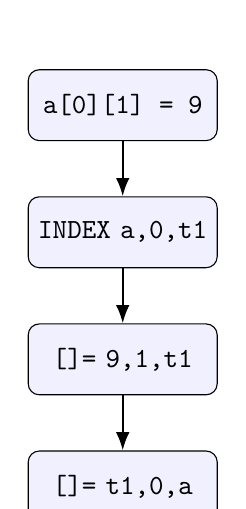
\begin{tikzpicture}[node distance=7mm and 10mm]
        \node[box] (src) {\pkg{a[0][1] = 9}};
        \node[box, below=of src] (i1) {\op{INDEX} \pkg{a,0,t1}};
        \node[box, below=of i1] (i2) {\op{[]=} \pkg{9,1,t1}};
        \node[box, below=of i2] (i3) {\op{[]=} \pkg{t1,0,a}};

        \draw[flow] (src) -- (i1);
        \draw[flow] (i1) -- (i2);
        \draw[flow] (i2) -- (i3);
    \end{tikzpicture}
    \caption{嵌套数组/元组左值的回写思路}
    \label{fig:writeback-template}
\end{figure}

若没有最后一步“把修改后的临时子结构重新写回父结构”，则 \pkg{a[0][1] = 9} 实际只改了临时变量 \pkg{t1}，原数组 \pkg{a} 不会更新。当前项目通过递归回写机制解决了这一问题，这是作业二中较有工程含量的一处实现。

\subsection{典型程序与四元式示例}

下面给出一个覆盖强制规则核心路径的示例程序：

\begin{lstlisting}[language=Rust,caption={覆盖函数、赋值、if 与 while 的示例程序}]
fn calc(mut a:i32, b:i32) -> i32 {
    let mut acc:i32;
    acc = a + b * 2;
    if acc > 10 {
        acc = acc - 1;
    }
    while acc != 0 {
        acc = acc - 1;
    }
    return acc;
}
\end{lstlisting}

根据当前实现，其典型四元式形态如下：

\begin{lstlisting}[style=textStyle,caption={示例程序的典型四元式形态}]
FUNC       calc _ _
PARAM_DECL a    i32 mut
PARAM_DECL b    i32 _
*          b    2   t1
+          a    t1  t2
=          t2   _   acc
>          acc  10  t3
IF_FALSE   t3   _   L1
-          acc  1   t4
=          t4   _   acc
LABEL      L1   _   _
LABEL      L2   _   _
!=         acc  0   t5
IF_FALSE   t5   _   L3
-          acc  1   t6
=          t6   _   acc
GOTO       _    _   L2
LABEL      L3   _   _
RETURN     acc  _   _
END_FUNC   calc _ _
\end{lstlisting}

该结果非常适合教学展示，因为它把高级语言中的运算优先级、条件跳转和循环结构全部展开为简单直观的中间步骤。

\section{Web 服务与可视化设计}

\subsection{后端 API 设计}

\pkg{Easy\_Server/src/main.rs} 使用 Axum 提供两个路由：

\begin{itemize}
    \item \pkg{GET /}：返回内嵌的 \pkg{index.html}；
    \item \pkg{POST /api/analyze}：接收源程序文本，返回 token、AST、词法错误、语法错误、语义错误与四元式。
\end{itemize}

响应结构 \pkg{AnalyzeResponse} 同时聚合三个阶段的结果，其主要字段如下：

\begin{itemize}
    \item \pkg{tokens}
    \item \pkg{ast}
    \item \pkg{lexerErrors}
    \item \pkg{parseError}
    \item \pkg{semanticErrors}
    \item \pkg{quadruples}
\end{itemize}

这样的接口设计直接服务于前端展示：用户点一次“分析”，即可在不同标签页切换查看 token 表、AST 树、四元式和错误信息，而不需要分别调用多个接口。

\subsection{前端展示设计}

根目录 \pkg{index.html} 当前实现了四个主要结果标签页：

\begin{enumerate}[label=\arabic*.]
    \item Token 表；
    \item AST 树；
    \item 四元式；
    \item 错误信息。
\end{enumerate}

从页面结构可以看出，前端并不试图重新解释编译规则，而只是把后端返回的数据做可视化排版。对课程项目而言，这种做法是正确的：编译逻辑必须唯一地存在于 Rust 代码中，前端应只承担展示职责。否则，一旦前端和后端对错误条件理解不一致，就会出现“后端说有错、前端显示没错”的不一致问题。

\subsection{为何需要 Web 可视化}

仅从命令行 JSON 输出也可以完成作业二功能，但 Web 展示有三个额外价值：

\begin{itemize}
    \item 更适合答辩和演示，便于老师快速观察 token、AST、错误与四元式之间的对应关系；
    \item 更适合调试复杂输入，例如数组、元组、嵌套循环等结构；
    \item 可以把“中间代码生成器”从纯后台逻辑变成更有可观察性的教学工具。
\end{itemize}

课程评分标准中提到“程序实例与结果截屏”，而当前 Web 页面的存在正是支撑这一要求的工程基础。

\section{测试体系与验证分析}

\subsection{测试文件组织}

当前 \pkg{Easy\_Analyzer/tests} 目录下保留了较丰富的测试集合，不仅包含覆盖课程规则的正式测试，还保留了多轮 triage/probe 类型的探索性测试。表 \ref{tab:test-suites} 概括了这些测试文件的职责。

\begin{table}[H]
    \centering
    \caption{\pkg{Easy\_Analyzer} 测试集合概览}
    \label{tab:test-suites}
    \begin{tabularx}{\textwidth}{P{4.1cm}Y Y}
        \toprule
        测试文件 & 主要用途 & 特点 \\
        \midrule
        \pkg{requirements\_coverage.rs} & 覆盖强制规则和部分扩展规则 & 面向课程验收的核心检查 \\
        \pkg{assignment2\_ppt\_matrix.rs} & 直接对照 PPT 规则矩阵 & 强调“规则-实现”映射 \\
        \pkg{ir\_interpreter.rs} & 用解释器执行四元式验证控制流与运算结果 & 检查 IR 的行为正确性 \\
        \pkg{bug\_fixes.rs} & 回归测试历史缺陷修复 & 保证修复不回退 \\
        \pkg{triage.rs}、\pkg{triage\_round3.rs}、\pkg{triage\_round3\_extra.rs}、\pkg{triage\_round4.rs} & 探测边界行为与潜在问题 & 偏研究与调试性质 \\
        \pkg{r4\_probe.rs}、\pkg{r5\_probe.rs}、\pkg{r6\_probe.rs} 等 & 某一轮复审的专项探测 & 用于定位复杂角落案例 \\
        \pkg{smoke.rs} & 基础冒烟检查 & 快速验证整体可用性 \\
        \bottomrule
    \end{tabularx}
\end{table}

从测试命名就能看出，当前项目并不是“只写了几条 happy path 用例”，而是把作业二视为一个需要持续收敛缺陷的工程系统。对于课程答辩，这一点非常有价值，因为它说明团队在实现过程中确实系统性地检查了规则边界，而不是仅靠少量示例拼凑出表面功能。

\subsection{强制规则覆盖验证}

\pkg{requirements\_coverage.rs} 和 \pkg{assignment2\_ppt\_matrix.rs} 是最能直接体现课程目标的两组测试。它们至少验证了以下方面：

\begin{itemize}
    \item 强制规则要求的函数、变量、表达式、\pkg{if} 与 \pkg{while} 能生成核心四元式；
    \item 形参与实参数量不一致、返回值类型不一致、变量未声明、变量未初始化、无返回值函数作右值等典型错误都能被报告；
    \item 扩展规则中的引用、数组、元组、\pkg{for}、\pkg{loop}、\pkg{break value} 等在多数代表性场景下可正常工作。
\end{itemize}

仓库 \pkg{README.md} 还记录了最近一次针对性测试结果：\pkg{requirements\_coverage} 为 8 个测试通过，\pkg{assignment2\_ppt\_matrix} 为 6 个测试通过，以下是测试结果运行：

\begin{figure}[htbp]
    \centering
    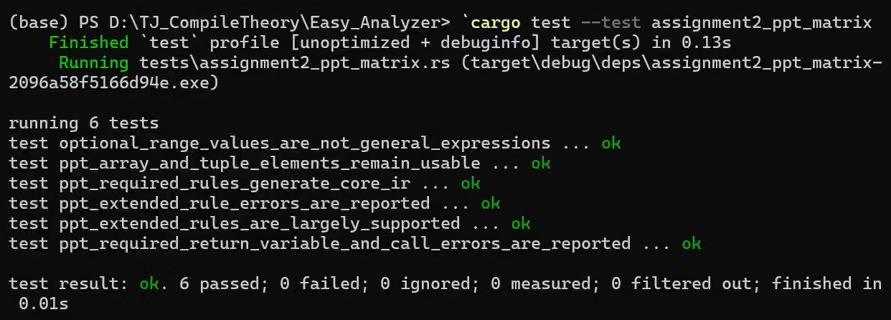
\includegraphics[width=0.8\textwidth]{figures/test1.jpg}
    \caption{requirements\_coverage 测试结果}
    \label{fig:test1}
\end{figure}

\begin{figure}[htbp]
    \centering
    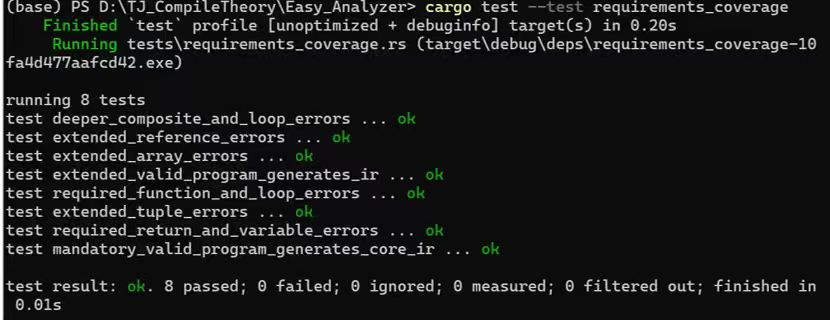
\includegraphics[width=0.8\textwidth]{figures/test2.jpg}
    \caption{assignment2\_ppt\_matrix 测试结果}
    \label{fig:test2}
\end{figure}

\subsection{IR 解释器验证的意义}

仅检查“生成了某些操作码”并不足以证明 IR 正确。例如，一个循环中即便出现了 \op{LABEL}、\op{IF\_FALSE} 和 \op{GOTO}，也可能因为标签位置不对而逻辑错误。为此，项目专门编写了 \pkg{ir\_interpreter.rs}，对生成的四元式做行为级验证。例如：

\begin{itemize}
    \item \pkg{break} 是否真的终止 \pkg{while}；
    \item \pkg{continue} 是否跳过当前迭代剩余语句；
    \item 嵌套循环中的 \pkg{break} 是否只影响最内层；
    \item \op{BREAK} 与 \op{CONTINUE} 四元式是否携带了正确目标标签。
\end{itemize}

这种“对 IR 再执行一遍”的测试策略非常有价值，因为它把“语法上看起来合理”的中间代码进一步提升为“语义上真正可执行”的中间代码。

\subsection{多轮缺陷修复与回归保障}

项目在 \pkg{Resources/Task2/bug\_report.md} 中保留了多轮复审记录，涉及 \pkg{break/continue} 标签、空数组处理、函数名作值、重复函数、数组和元组写回、\pkg{for continue} 死循环、静态越界检查、\pkg{i32::MIN} 负字面量等多个问题。虽然这些问题中的大多数已经修复，但它们有两个重要意义：

\begin{enumerate}[label=\arabic*.]
    \item 说明语义分析与 IR 生成并非“写完就对”，而是需要通过系统性测试逐步打磨；
    \item 每个修复点都对应了具体回归测试，从而避免未来改动把旧缺陷重新引入。
\end{enumerate}

从软件工程角度看，这种“问题单 $\rightarrow$ 修复 $\rightarrow$ 回归测试”的闭环，正是课程项目从“作业代码”迈向“有维护意识的工程实现”的体现。

\section{作业要求与当前实现的对照分析}

\subsection{强制规则对照说明}

课程验收首先看强制规则是否完整覆盖。从当前实现与测试文件可见，强制规则已经在三个层面落实：

\begin{itemize}
    \item 语法层：相关构造能够被 lexer 和 parser 正确识别；
    \item 语义层：相关静态约束能够被 analyzer 检查；
    \item 中间代码层：合法构造能够生成结构合理的四元式。
\end{itemize}

例如，规则 3.5 并不是“能写出调用语法”就算完成，而是要求调用能做参数数量检查、参数类型检查、返回值位置处理，并在无返回值函数作右值时报告错误。当前实现正是按照这种较完整的标准来覆盖规则的。

\subsection{扩展规则完成度分析}

虽然 PPT 明确说剩余规则不做强制要求，但当前项目并没有停留在最低线，而是继续支持了：

\begin{itemize}
    \item \pkg{else} 与 \pkg{else if}
    \item \pkg{for}、\pkg{loop}、\pkg{break}、\pkg{continue}
    \item 不可变变量、引用、可变引用、解引用
    \item 表达式块、\pkg{if} 表达式、\pkg{loop} 表达式
    \item 数组类型、数组字面量、数组元素访问
    \item 元组类型、元组字面量、元组字段访问
\end{itemize}

这说明当前实现已经不仅仅是“通过验收”，而是有一定完整性的课程级语义前端原型。

\section{存在的限制与后续改进方向}

\subsection{当前实现的主要限制}

尽管当前实现已经较完整，但与真正的 Rust 编译器相比，仍有一些明确限制：

\begin{enumerate}[label=\arabic*.]
    \item \pkg{a..b} 范围主要服务于 \pkg{for}，并不是普通一等表达式；
    \item 借用检查是课程级简化版本，没有实现完整生命周期、移动语义和别名分析；
    \item 语言没有布尔字面量、逻辑与或、字符串、结构体、模式匹配、泛型、闭包等更完整特性；
    \item 顶层仓库尚未组织为统一 workspace，构建与测试需要分别进入各 crate；
    \item Web 界面当前更偏展示型工具，对 API 自身的自动化测试还可进一步增强。
\end{enumerate}

这些限制中，有些是课程范围刻意收缩的结果，有些则是后续若继续迭代可以逐步补强的工程点。

\subsection{可继续深化的方向}

若以后继续扩展本项目，可以优先考虑以下几个方向：

\begin{itemize}
    \item 把四元式再进一步规范为基本块或 SSA 形式，为优化做准备；
    \item 为错误结构增加更精细的位置信息与规则编号，提升前端诊断体验；
    \item 增加逻辑运算与短路求值，完善布尔类型体系；
    \item 增加更严格的借用生命周期分析，使引用语义更接近真实 Rust；
    \item 将各 crate 组织为 workspace，并补充端到端自动化测试。
\end{itemize}

这些改进并不意味着当前实现“还不够像编译器”，而是说明课程项目已经具备继续生长的技术基础。

\section{总结}

综合来看，当前仓库中的作业二实现已经形成了一个结构清晰、职责明确、具备一定工程质量的类 Rust 语义分析与四元式中间代码生成器。它以作业一的词法分析与语法分析为基础，完成了从 AST 到语义结果、从语义结果到四元式的进一步推进，覆盖了课程强制要求的全部规则，并对引用、表达式块、数组、元组、\pkg{for}、\pkg{loop} 等扩展规则进行了较完整实现。

从设计角度看，本项目的优势主要体现在以下几点：

\begin{itemize}
    \item 采用分层式实现，将 AST、内部类型系统、符号表、循环上下文与 IR 生成清晰拆分；
    \item 对强制规则并非停留在“能过语法”，而是真正落到了静态语义检查与中间代码模板中；
    \item 通过 \pkg{Type::Unknown}、\pkg{Type::Never}、\pkg{Type::Error} 等设计提高了错误恢复与表达能力；
    \item 借助 Web 服务、前端界面与 IR 解释器，使结果具备良好的可观察性和验证性；
    \item 通过较系统的测试与缺陷回归，将课程项目提升到“可以被持续维护”的工程水平。
\end{itemize}

因此，若从课程作业 2 的要求出发，本文所分析的当前实现已经不仅能完成“最小中间代码生成器”的任务，而且展示了较强的问题分析能力和系统化设计思路。它既适合作为课程答辩中的展示样例，也具有继续向后扩展为更完整教学编译器的潜力。

\appendix

\section{附录 A：强制规则实现对照表}

\begin{longtable}{P{1.4cm}P{4.2cm}P{4.4cm}P{3.8cm}}
    \caption{强制规则实现对照表}\label{tab:mandatory-matrix}\\
    \toprule
    规则 & 要求摘要 & 当前实现位置 & 说明 \\
    \midrule
    \endfirsthead
    \toprule
    规则 & 要求摘要 & 当前实现位置 & 说明 \\
    \midrule
    \endhead
    0.1 & \pkg{mut} 可变属性 & \pkg{Binding.mutable}、\pkg{VarSymbol.mutable}、\pkg{gen\_assign()} & 允许二次赋值与参数可变性记录 \\
    0.2 & \pkg{i32} 基础类型 & \pkg{Type::I32}、数字字面量检查 & 统一整数语义与越界检查 \\
    0.3 & 左值与标识符属性 & \pkg{Expr::is\_assignable()}、\pkg{gen\_assign()} & 支持标识符、解引用、下标、字段作为左值 \\
    1.1 & 基础程序与函数声明 & \pkg{Program}、\pkg{FunctionDecl}、\pkg{analyze\_program()} & 先收集函数签名再分析函数体 \\
    1.2 & 语句与空语句 & \pkg{Statement::Empty}、\pkg{gen\_stmt()} & 空语句直接跳过 \\
    1.3 & \pkg{return;} & \pkg{gen\_return()} & 与函数声明返回类型联合检查 \\
    1.4 & 函数输入参数 & \pkg{parse\_parameter\_list()}、\pkg{build\_function\_sig()} & 检查参数类型、重名与可变性 \\
    1.5 & 函数输出与 \pkg{return expr;} & \pkg{gen\_return()}、函数尾表达式处理 & 检查返回类型一致性 \\
    2.0 & 变量声明 & \pkg{Binding}、\pkg{VarSymbol} & 支持显式类型和待推断声明 \\
    2.1 & \pkg{let} 声明语句 & \pkg{Statement::Let}、\pkg{gen\_let()} & 支持 shadowing 与作用域结束时推断检查 \\
    2.2 & 赋值语句 & \pkg{gen\_assign()} & 同时检查声明、初始化、可变性和类型匹配 \\
    3.1 & 基本表达式 & \pkg{gen\_expr\_inner()} & 支持数字、变量、括号表达式 \\
    3.2 & 比较运算 & \pkg{gen\_binary()} & 结果类型为 \pkg{Bool} \\
    3.3 & 加减运算 & \pkg{gen\_binary()} & 以四元式方式生成临时结果 \\
    3.4 & 乘除运算 & \pkg{gen\_binary()} & 优先级高于加减 \\
    3.5 & 函数调用 & \pkg{gen\_call()} & 检查函数声明、参数数量、参数类型与返回值位置 \\
    4.1 & \pkg{if} 选择结构 & \pkg{gen\_if\_expr()} & 支持语句与表达式两用 \\
    5.0 & 循环语句框架 & \pkg{FuncCtx.loop\_depth}、\pkg{LoopLabels} & 统一支撑 \pkg{while}/\pkg{for}/\pkg{loop} \\
    5.1 & \pkg{while} 循环 & \pkg{gen\_while()} & 发射 \op{LABEL}、\op{IF\_FALSE}、\op{GOTO} \\
    \bottomrule
\end{longtable}

\section{附录 B：扩展规则实现对照表}

\begin{longtable}{P{1.6cm}P{4.1cm}P{4.5cm}P{3.6cm}}
    \caption{扩展规则实现对照表}\label{tab:extended-matrix}\\
    \toprule
    规则 & 要求摘要 & 当前实现位置 & 说明 \\
    \midrule
    \endfirsthead
    \toprule
    规则 & 要求摘要 & 当前实现位置 & 说明 \\
    \midrule
    \endhead
    2.3 & 声明同时初始化 & \pkg{gen\_let()} & 支持类型推断与显式类型匹配 \\
    4.2 & \pkg{else} & \pkg{ElseBranch::Block}、\pkg{gen\_if\_expr()} & 生成 else 分支与合流标签 \\
    4.3 & \pkg{else if} & \pkg{ElseBranch::ElseIf} & 递归复用 \pkg{if} 表达式逻辑 \\
    5.2 & \pkg{for} 循环 & \pkg{gen\_for()} & 支持范围与数组迭代 \\
    5.3 & \pkg{loop} & \pkg{Expr::Loop}、\pkg{gen\_loop\_expr()} & 支持无限循环与表达式语义 \\
    5.4 & \pkg{break}/\pkg{continue} & \pkg{gen\_break()}、\pkg{gen\_continue()} & 标签化跳转并支持 \pkg{break value} \\
    6.1 & 不可变变量 & \pkg{gen\_assign()} & 初次初始化后禁止二次赋值 \\
    6.2 & 不可变引用 & \pkg{UnaryOp::Ref}、\pkg{register\_borrow()} & 允许多个共享引用 \\
    6.3 & 可变引用 & \pkg{UnaryOp::RefMut}、借用冲突检查 & 独占借用，要求根变量可变 \\
    6.4 & 解引用 & \pkg{UnaryOp::Deref}、\pkg{*=} & 支持读写并区分可变性 \\
    7.0 & 表达式块 & \pkg{Block.tail}、\pkg{gen\_block\_expr()} & 局部作用域与尾表达式返回值 \\
    7.1 & 块作为表达式 & \pkg{Expr::Block} & 可作为右值参与计算 \\
    7.2 & 块作为函数体 & \pkg{FunctionDecl.body} & 尾表达式可作为隐式返回 \\
    7.3 & \pkg{if} 表达式 & \pkg{gen\_if\_expr()} & 支持分支值合流 \\
    7.4 & \pkg{loop} 表达式 & \pkg{gen\_loop\_expr()}、\pkg{gen\_break()} & 用 \pkg{break value} 产生结果值 \\
    8.1 & 数组类型 & \pkg{Type::Array}、\pkg{validate\_type()} & 检查长度为正整数常量 \\
    8.2 & 数组字面量 & \pkg{gen\_array()} & 检查元素类型与长度一致性 \\
    8.3 & 数组元素 & \pkg{gen\_index()}、\pkg{check\_array\_static\_oob()} & 支持读取、写回与静态越界检查 \\
    9.1 & 元组类型 & \pkg{Type::Tuple} & 支持空元组、单元素元组与多元素元组 \\
    9.2 & 元组字面量 & \pkg{gen\_tuple()} & 检查元素个数与类型一致性 \\
    9.3 & 元组字段 & \pkg{gen\_field()}、\pkg{.=} & 支持字段读取、写回与越界检查 \\
    \bottomrule
\end{longtable}

\section{附录 C：典型源码片段与分析说明}

\subsection{函数调用与返回值检查示例}

\begin{lstlisting}[language=Rust,caption={函数调用规则示例}]
fn add(mut a:i32, b:i32) -> i32 {
    return a + b;
}

fn main() {
    let answer:i32 = add(1, 2);
}
\end{lstlisting}

该示例同时覆盖了函数声明、参数类型、返回值类型、算术运算和函数调用，是课程 PPT 强制规则路径中的典型正例。

\subsection{引用与解引用示例}

\begin{lstlisting}[language=Rust,caption={引用、可变引用与解引用示例}]
fn main() {
    let mut a:i32 = 1;
    let p:&mut i32 = &mut a;
    *p = 2;
}
\end{lstlisting}

这个例子展示了扩展规则 6.2、6.3 和 6.4 的联合工作方式：首先从可变变量创建可变引用，然后通过解引用完成写入。

\subsection{数组与元组示例}

\begin{lstlisting}[language=Rust,caption={数组与元组组合示例}]
fn main() {
    let mut arr:[i32;3] = [1, 2, 3];
    arr[1] = arr[0] + 2;

    let mut pair:(i32, i32) = (arr[0], arr[1]);
    pair.0 = pair.1;
}
\end{lstlisting}

该示例能够很好地展示数组下标读取/写回、元组字段读取/写回以及嵌套表达式求值的四元式形态。

\section{附录 D：测试与工程演进补充说明}

为了保证作业二实现不是一次性“写完即交”的代码，项目保留了较完整的工程演进轨迹：

\begin{itemize}
    \item \pkg{bug\_report.md} 汇总了多轮 BUG 复审结论，覆盖控制流标签、数组与元组写回、函数名作值、静态越界、\pkg{i32::MIN} 等问题；
    \item \pkg{discussions.md} 记录了若干设计取舍，包括严格条件类型、\pkg{Never} 类型、静态越界策略、函数值绑定等；
    \item 各轮 triage/probe 测试保留了大量探索性案例，帮助识别课程规则边缘与工程化问题。
\end{itemize}

从课程报告写作角度看，这些文件的意义不只是“证明写过测试”，而是说明实现过程本身具备分析、迭代、修复和回归的完整链条。这一点与评分标准中的“问题分析能力”和“系统方案设计能力”高度一致。

\begin{thebibliography}{99}

\bibitem{dragonbook}
Alfred V. Aho, Monica S. Lam, Ravi Sethi, Jeffrey D. Ullman.
\newblock \emph{Compilers: Principles, Techniques, and Tools}.
\newblock Pearson, 2nd Edition, 2006.

\bibitem{engineering}
Keith D. Cooper, Linda Torczon.
\newblock \emph{Engineering a Compiler}.
\newblock Morgan Kaufmann, 2nd Edition, 2011.

\bibitem{rustbook}
Steve Klabnik, Carol Nichols.
\newblock \emph{The Rust Programming Language}.
\newblock No Starch Press, 2nd Edition, 2019.

\bibitem{rustref}
The Rust Project Developers.
\newblock \emph{The Rust Reference}.
\newblock \url{https://doc.rust-lang.org/reference/}

\bibitem{courseppt}
同济大学编译原理课程组.
\newblock 《【Rust版】大作业2：中间代码生成器》课程 PPT.
\newblock 课程资源文件，位于 \pkg{Resources/Task2} 目录.

\bibitem{repo}
TJ\_CompileTheory 项目仓库源码与测试文件.
\newblock 包括 \pkg{README.md}、\pkg{Easy\_Analyzer/src} 与 \pkg{Easy\_Analyzer/tests}.

\end{thebibliography}

\end{document}
